\begin{figure*}[!t]
\centering
\resizebox{\textwidth}{!}{%
\begin{tikzpicture}[
    node distance=0.4cm and 0.6cm,
    stage/.style={draw, rounded corners=4pt, minimum height=1.1cm, minimum width=2.0cm, align=center, font=\footnotesize, inner sep=5pt, thick},
    io/.style={draw, rounded corners=3pt, minimum height=0.7cm, minimum width=1.4cm, align=center, font=\footnotesize, inner sep=3pt, fill=black!5},
    smallio/.style={draw, rounded corners=3pt, minimum height=0.6cm, align=center, font=\scriptsize, inner sep=3pt, fill=black!5},
    detail/.style={font=\tiny, text=black!50, align=center},
    arr/.style={-{Stealth[length=2.5mm]}, thick},
    grouplabel/.style={font=\footnotesize\bfseries\sffamily, text=black!60},
    inputtag/.style={draw, rounded corners=2pt, fill=white, font=\tiny, inner sep=2pt, minimum height=0.4cm},
]

% =====================================================
% ROW 1: Registry Pipeline (wider spacing for centering)
% =====================================================
\node[io] (input) {Crop +\\disease list};
\node[stage, right=0.7cm of input, fill=blue!8] (disc) {{\small\faSearch}\\[1pt]\textbf{Discovery}};
\node[detail, below=0.15cm of disc] (disc_d) {web search\\per disease};
\node[stage, right=0.7cm of disc, fill=orange!10] (ext) {{\small\faGlobe}\\[1pt]\textbf{Extraction}};
\node[detail, below=0.15cm of ext] (ext_d) {1 URL/call\\verbatim quotes};
\node[stage, right=0.7cm of ext, fill=purple!8] (rec) {{\small\faCodeBranch}\\[1pt]\textbf{Reconciliation}};
\node[detail, below=0.15cm of rec] (rec_d) {LLM cross-source\\merge + normalize};

% Expert evidence audit — manual review of cited verbatim quotes per KB field
\node[stage, right=0.7cm of rec, fill=red!6] (expert_kb) {{\small\faUserCheck}\\[1pt]\textbf{Expert Audit}};
\node[detail, below=0.15cm of expert_kb] (expert_kb_d) {evidence audit\\per KB field};

% KB output (covers all crops in the dataset; counts from Table 1)
\node[draw, rounded corners=4pt, right=0.7cm of expert_kb, fill=green!6, minimum width=2.4cm, minimum height=1.1cm, align=center, font=\scriptsize, inner sep=4pt, thick] (kb) {
    {\small\faBookOpen}\\[1pt]
    \textbf{Canonical KB}\\[1pt]
    {\tiny 335 crops $\cdot$ 1{,}251 diseases}\\[-1pt]
    {\tiny cited symptom text}
};

\draw[arr] (input) -- (disc);
\draw[arr] (disc) -- (ext);
\draw[arr] (ext) -- (rec);
\draw[arr] (rec) -- (expert_kb);
\draw[arr] (expert_kb) -- (kb);

% =====================================================
% ROW 2: Image Filtering (wider spacing)
% =====================================================
\node[io, below=1.6cm of input, align=center] (rawimg) {{\small\faImages}\\Raw images\\[-1pt]{\tiny\color{black!60}$\sim$839K, multi-source}};

% Expert dedupe — collapse cross-source class-name variants (e.g., "Leaf Rust" vs "leaf_rust")
\node[stage, right=0.7cm of rawimg, fill=red!6] (expert_img) {{\small\faUserCheck}\\[1pt]\textbf{Expert Dedupe}};
\node[detail, below=0.15cm of expert_img] (expert_img_d) {cross-source\\class name dedupe};

\node[stage, right=0.7cm of expert_img, fill=teal!10] (filter) {{\small\faFilter}\\[1pt]\textbf{Image Filtering}\\{\tiny VLM + KB symptoms}};
\node[detail, below=0.15cm of filter] (filter_d) {match/reject per image\\+ organ tagging};

% Ref set and Test set stacked vertically; Anat. index to the right
\node[smallio, right=1.2cm of filter, yshift=0.35cm] (refs) {{\scriptsize\faThLarge}~Reference Set};
\node[smallio, below=0.25cm of refs] (testset) {{\scriptsize\faImage}~Test Set};
\node[draw, rounded corners=3pt, fill=yellow!10, right=0.8cm of refs, align=left, font=\scriptsize, inner sep=4pt] (anatidx) {%
    {\scriptsize\faSitemap}~\textbf{Anatomical Index}\\[1pt]
    {\tiny\color{black!65} leaf \,\textbar\, stem \,\textbar\, root \,\textbar\, fruit \,\textbar\, seed \,\textbar\, pod}%
};

\draw[arr] (rawimg) -- (expert_img);
\draw[arr] (expert_img) -- (filter);
\draw[arr] (filter) -- (refs);
\draw[arr] (filter) -- (testset);
% Anat. index derived from ref set
\draw[arr] (refs) -- (anatidx);
% KB→filter: route ABOVE the output nodes (refs/testset/anatidx)
% Horizontal segment runs 0.35cm above filter.north, clearing the output row
\coordinate (kb_route) at ($(filter.north)+(0.3,0.35)$);
\draw[arr, black!40] (kb.south) |- (kb_route) -- ($(filter.north)+(0.3,0)$);

% =====================================================
% Dedicated Regional (Delta) KB sub-pipeline — multi-agent swarm
% Visualizes per-(disease, state) delta extraction by a VLM swarm.
% =====================================================
% Stacked "shadow" boxes behind the swarm node convey N parallel agents.
\node[draw, rounded corners=4pt, below=0.9cm of filter, fill=purple!6,
      align=center, font=\scriptsize, inner sep=5pt, very thick, draw=purple!50] (swarm) {
    {\small\faRobot}~\textbf{VLM Swarm}\;\,{\tiny\color{black!55}organ-routed, 24 specialists}\\[1pt]
    {\tiny\bfseries 2 rounds $\cdot$ peer blackboard (support / challenge / withdraw)}\\[3pt]
    \setlength{\tabcolsep}{2pt}\renewcommand{\arraystretch}{1.1}%
    \begin{tabular}{cccc}
      \fcolorbox{black!35}{green!12}{\tiny\faLeaf\ Leaf $\times8$} &
      \fcolorbox{black!35}{orange!12}{\tiny\faSeedling\ Stem $\times4$} &
      \fcolorbox{black!35}{teal!12}{\tiny\faCarrot\ Below-ground $\times2$} &
      \fcolorbox{black!35}{red!10}{\tiny\faSpa\ Reproductive $\times2$} \\
      \fcolorbox{black!35}{purple!12}{\tiny\faBug\ Signs $\times1$} &
      \fcolorbox{black!35}{blue!10}{\tiny\faTree\ Whole-plant $\times3$} &
      \multicolumn{2}{c}{\fcolorbox{black!35}{yellow!16}{\tiny\faMicroscope\ Cross-cutters $\times4$}} \\
    \end{tabular}\\[2pt]
    {\tiny organ router $\to$ specialists $\to$ \textbf{VisualDiagnosis} consolidator}
};
\node[detail, below=0.12cm of swarm] (swarm_d) {per (disease, state) $\cdot$ consensus delta};
\node[draw, rounded corners=4pt, right=0.9cm of swarm, fill=orange!14,
      minimum width=2.5cm, minimum height=1.15cm, align=center, font=\scriptsize,
      inner sep=4pt, very thick, draw=orange!55!black] (regkb) {
    {\small\faGlobe}\\[1pt]
    \textbf{Regional Delta KB}\\[-1pt]
    {\tiny dedicated, per (disease, state)}\\[-1pt]
    {\tiny image-grounded}
};
% filtered field images -> swarm -> regional KB; canonical text grounds the deltas
\draw[arr] (filter.south) -- (swarm.north);
\draw[arr] (swarm) -- (regkb);
\draw[arr, densely dashed, black!45] (kb.east) to[out=0,in=60] (regkb.north east)
  node[midway, font=\tiny, text=black!55, fill=white, inner sep=1pt] {grounds};

% (Curation and inference backgrounds drawn after all nodes are placed)

% =====================================================
% ROW 3: Agentic Diagnostic Flow
% Positioned with extra gap below curation box
% =====================================================

% Test image — anchor to left, well below curation box (extra gap)
\node[draw, rounded corners=3pt, below=6.4cm of rawimg, fill=black!5, minimum width=1.6cm, align=center, font=\scriptsize, inner sep=4pt] (agentinputs) {
    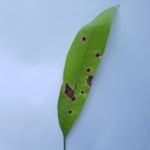
\includegraphics[width=1.1cm, height=1.1cm]{figures/sample_test_mango.jpg}\\[2pt]
    {\tiny Test image}
};

% Step 1: Observe
\node[stage, right=0.7cm of agentinputs, fill=blue!6, minimum width=2.0cm] (observe) {
    {\small\faEye}\\[1pt]
    \textbf{Encoder}\\[-1pt]
    {\tiny frozen BioCLIP}
};
\node[detail, below=0.15cm of observe] (obs_d) {image embedding};

% Step 2: Anatomical narrowing
\node[stage, right=0.7cm of observe, fill=yellow!12, minimum width=2.2cm] (narrow) {
    {\small\faThList}\\[1pt]
    \textbf{Prototype}\\[-1pt]
    {\tiny short-list (top-5)}
};
\node[detail, below=0.15cm of narrow] (narrow_d) {recall@5 $\approx$ \textbf{ceiling}};

% Step 3: KB reasoning
\node[stage, right=0.7cm of narrow, fill=green!8, minimum width=2.0cm] (kbreason) {
    {\small\faSearch}\\[1pt]
    \textbf{Adaptive}\\[-1pt]
    {\tiny retrieve $k$ cases}
};
\node[detail, below=0.15cm of kbreason] (kbr_d) {labels$+$sim \emph{as text}};

% Step 4: Visual comparison
\node[draw, rounded corners=4pt, right=0.7cm of kbreason, fill=purple!8, minimum width=2.8cm, minimum height=1.4cm, align=center, thick] (compare) {
    \textbf{{\small\faRobot}~Text-only LLM}\\[3pt]
    {\scriptsize re-ranks short-list using}\\[-1pt]
    {\scriptsize retrieved labels $+$ Delta-KB symptoms}\\[3pt]
    {\tiny\bfseries\color{purple!60!black} never sees a pixel}
};

% Step 5: Prediction + trace
\node[draw, rounded corners=4pt, right=0.6cm of compare, fill=green!15, minimum width=1.8cm, minimum height=1.2cm, align=center, font=\footnotesize, inner sep=4pt, thick] (pred) {
    {\small\faCheckCircle}\\[1pt]
    \textbf{Prediction}\\[1pt]
    {\tiny\textit{Anthracnose}}\\[-1pt]
    {\tiny + reasoning trace}
};

% Input tags — top-right corner, anchored relative to pred (now defined)
\node[inputtag, fill=orange!12, above=1.0cm of pred] (intag_anat) {{\tiny\faDatabase}~Delta KB};
\node[inputtag, fill=black!5, left=0.25cm of intag_anat] (intag_refs) {{\tiny\faThLarge}~Prototype pool};
\node[inputtag, fill=green!8, left=0.25cm of intag_refs] (intag_kb) {{\tiny\faBookOpen}~Canonical KB};
\node[draw=black!25, rounded corners=4pt, inner sep=5pt, densely dashed,
      fit=(intag_kb)(intag_refs)(intag_anat),
      label={[font=\tiny\bfseries\sffamily, text=black!50, anchor=south]above:{\faArrowDown} from Curation}] (inputsbox) {};

% Row 3 horizontal arrows
\draw[arr] (agentinputs) -- (observe);
\draw[arr] (observe) -- (narrow);
\draw[arr] (narrow) -- (kbreason);
\draw[arr] (kbreason) -- (compare);
\draw[arr] (compare) -- (pred);

% Open-ended reasoning loop: Compare -> back to KB Lookup, bounded by k references
\coordinate (loopL) at ($(compare.north)+(0,0.55)$);
\coordinate (loopR) at ($(kbreason.north)+(0,0.55)$);
\draw[arr, densely dashed, black!55, rounded corners=4pt]
    (compare.north) -- (loopL) -- (loopR) -- (kbreason.north);
\node[font=\tiny\itshape, text=black!60, anchor=north]
    at ($(loopL)!0.5!(loopR)+(0,-0.05)$) {$k$ retrieved labels (text)};

% Dashed rectangle around reasoning steps (open-ended loop)
\begin{scope}[on background layer]
    \node[draw=black!30, dashed, rounded corners=6pt, inner sep=10pt,
          fit=(observe)(narrow)(kbreason)(compare)(obs_d)(narrow_d)(kbr_d),
          label={[font=\tiny\itshape, text=black!45]above:text-only reasoning $\cdot$ no pixels to the LLM $\cdot$ evidence budget $k$}] (reasonbox) {};
\end{scope}

% =====================================================
% Reasoning-trace strip — one step from a real trace
% (Mango Anthracnose, sonnet+KB, k=4 — from trace_appendix_13.tex)
% Framed as prev / current / next to convey step-by-step nature
% =====================================================
\node[draw=black!25, fill=blue!2, rounded corners=4pt,
      below=0.05cm of reasonbox.south, inner sep=3pt,
      font=\scriptsize, align=left, text width=14.0cm] (tracestrip) {%
    {\tiny\bfseries\sffamily\color{black!60} EXAMPLE (text-only LLM)}\,\,\textbar\,\,
    {\tiny mango,\, encoder short-list $+$ Delta-KB,\, $k{=}4$}%
    \hfill{\tiny\sffamily\color{black!55} no image reads}\\[1pt]
    {\color{black!20}\hrulefill}\\[1pt]
    {\scriptsize\color{black!50}\textbf{short-list}\,:}\, Anthracnose (0.41), Sooty Mould (0.22), Bacterial Spot (0.14), \dots\\[2pt]
    {\scriptsize\color{black!85}\textbf{LLM}\,:}\, \textit{``3 of 4 retrieved neighbours are labelled Anthracnose; Delta-KB notes \emph{discrete} dark spots, not the \emph{diffuse} coating of Sooty Mould.''}\\[2pt]
    {\scriptsize\color{black!50}\textbf{decide}\,:}\, promote rank-1\hfill$\Rightarrow$ \textbf{Anthracnose} \textcolor{green!55!black}{\faCheckCircle}\,Correct%
};
% Faint dotted leader from prediction down into the trace strip
\draw[densely dotted, black!35] (pred.south) -- ($(tracestrip.north -| pred.south)$);

% =====================================================
% VLM AGENT background (row 3 + input tags)
% Force same width as curation box using min width
% =====================================================
% =====================================================
% Draw BOTH background boxes with shared width
% (All nodes are now placed, so we can measure both)
% =====================================================
% Invisible fits to measure natural bounds of each group
\begin{scope}[on background layer]
    \node[draw=none, fill=none, inner sep=10pt,
          fit=(input)(kb)(rawimg)(anatidx)(filter)(disc_d)(ext_d)(rec_d)(expert_kb)(expert_kb_d)(expert_img)(expert_img_d)(filter_d)] (prepgroup_nat) {};
    \node[draw=none, fill=none, inner sep=10pt,
          fit=(swarm)(swarm_d)(regkb)] (reggroup_nat) {};
    \node[draw=none, fill=none, inner sep=10pt,
          fit=(agentinputs)(pred)(reasonbox)(obs_d)(narrow_d)(kbr_d)(inputsbox)(tracestrip)] (infgroup_nat) {};
\end{scope}

% Pick the leftmost left and rightmost right across all three groups
\path let \p1=(prepgroup_nat.west), \p2=(infgroup_nat.west), \p3=(reggroup_nat.west) in
      coordinate (sl) at ({min(\x1,\x2,\x3)}, 0);
\path let \p1=(prepgroup_nat.east), \p2=(infgroup_nat.east), \p3=(reggroup_nat.east) in
      coordinate (sr) at ({max(\x1,\x2,\x3)}, 0);

\begin{scope}[on background layer]
    % Invisible anchors at shared edges, projected to each group's vertical center
    \node[draw=none, fill=none, inner sep=0pt] at (sl |- prepgroup_nat.center) (cur_l) {};
    \node[draw=none, fill=none, inner sep=0pt] at (sr |- prepgroup_nat.center) (cur_r) {};
    \node[draw=none, fill=none, inner sep=0pt] at (sl |- reggroup_nat.center) (reg_l) {};
    \node[draw=none, fill=none, inner sep=0pt] at (sr |- reggroup_nat.center) (reg_r) {};
    \node[draw=none, fill=none, inner sep=0pt] at (sl |- infgroup_nat.center) (inf_l) {};
    \node[draw=none, fill=none, inner sep=0pt] at (sr |- infgroup_nat.center) (inf_r) {};

    % Curation box — content centered within shared width
    \node[draw=black!12, fill=black!3, rounded corners=8pt, inner sep=10pt,
          fit=(input)(kb)(rawimg)(anatidx)(filter)(disc_d)(ext_d)(rec_d)(expert_kb)(expert_kb_d)(expert_img)(expert_img_d)(filter_d)(cur_l)(cur_r)] (prepgroup) {};
    \node[grouplabel, anchor=north west] at ($(prepgroup.north west)+(0.15,-0.05)$) {{\small\faLayerGroup}~\textsc{Curation}};

    % Regional Delta-KB Collection box — its own tier between curation and inference
    \node[draw=orange!35, fill=orange!4, rounded corners=8pt, inner sep=10pt,
          fit=(swarm)(swarm_d)(regkb)(reg_l)(reg_r)] (reggroup) {};
    \node[grouplabel, anchor=north west, text=orange!50!black] at ($(reggroup.north west)+(0.15,-0.05)$) {{\small\faGlobe}~\textsc{Regional Delta-KB Collection}};

    % Inference box — same shared width
    \node[draw=blue!20, fill=blue!4, rounded corners=8pt, inner sep=10pt,
          fit=(agentinputs)(pred)(reasonbox)(obs_d)(narrow_d)(kbr_d)(inputsbox)(tracestrip)(inf_l)(inf_r)] (infgroup) {};
    \node[grouplabel, anchor=north west, text=blue!50!black] at ($(infgroup.north west)+(0.15,-0.05)$) {{\small\faRobot}~\textsc{Cost-Effective Retrieval--Reasoning Inference} {\normalfont\footnotesize (\$5 sweep vs.\ \$18--35/crop)}};
\end{scope}

\end{tikzpicture}
}%
\caption{\textbf{\textsc{Presage} overview.} \textbf{Curation} (top): web pages
become a source-cited canonical KB (335 crops, 1{,}251 diseases) with an expert
audit; geo-tagged field images are deduped, filtered, and---per (disease,
state)---captioned by a VLM into image-grounded \emph{deltas}.
\textbf{Cost-effective inference} (bottom): we factor perception from
reasoning. A frozen encoder embeds the test image into an image-prototype
short-list (near-ceiling recall@5); the $k$ visually nearest labelled cases are
retrieved \emph{adaptively} and passed---as label$+$similarity \emph{text}---to
a language model that re-ranks using that evidence plus Delta-KB symptoms. The
LLM \textbf{never sees a pixel}, cutting per-crop cost from \$18--35
(image-streaming agents) to a few dollars for the entire sweep.}
\label{fig:teaser}
\end{figure*}
